% Options for packages loaded elsewhere
\PassOptionsToPackage{unicode}{hyperref}
\PassOptionsToPackage{hyphens}{url}
%
\documentclass[
]{article}
\usepackage{amsmath,amssymb}
\usepackage{iftex}
\ifPDFTeX
  \usepackage[T1]{fontenc}
  \usepackage[utf8]{inputenc}
  \usepackage{textcomp} % provide euro and other symbols
\else % if luatex or xetex
  \usepackage{unicode-math} % this also loads fontspec
  \defaultfontfeatures{Scale=MatchLowercase}
  \defaultfontfeatures[\rmfamily]{Ligatures=TeX,Scale=1}
\fi
\usepackage{lmodern}
\ifPDFTeX\else
  % xetex/luatex font selection
\fi
% Use upquote if available, for straight quotes in verbatim environments
\IfFileExists{upquote.sty}{\usepackage{upquote}}{}
\IfFileExists{microtype.sty}{% use microtype if available
  \usepackage[]{microtype}
  \UseMicrotypeSet[protrusion]{basicmath} % disable protrusion for tt fonts
}{}
\makeatletter
\@ifundefined{KOMAClassName}{% if non-KOMA class
  \IfFileExists{parskip.sty}{%
    \usepackage{parskip}
  }{% else
    \setlength{\parindent}{0pt}
    \setlength{\parskip}{6pt plus 2pt minus 1pt}}
}{% if KOMA class
  \KOMAoptions{parskip=half}}
\makeatother
\usepackage{xcolor}
\usepackage[margin=1in]{geometry}
\usepackage{graphicx}
\makeatletter
\def\maxwidth{\ifdim\Gin@nat@width>\linewidth\linewidth\else\Gin@nat@width\fi}
\def\maxheight{\ifdim\Gin@nat@height>\textheight\textheight\else\Gin@nat@height\fi}
\makeatother
% Scale images if necessary, so that they will not overflow the page
% margins by default, and it is still possible to overwrite the defaults
% using explicit options in \includegraphics[width, height, ...]{}
\setkeys{Gin}{width=\maxwidth,height=\maxheight,keepaspectratio}
% Set default figure placement to htbp
\makeatletter
\def\fps@figure{htbp}
\makeatother
\setlength{\emergencystretch}{3em} % prevent overfull lines
\providecommand{\tightlist}{%
  \setlength{\itemsep}{0pt}\setlength{\parskip}{0pt}}
\setcounter{secnumdepth}{-\maxdimen} % remove section numbering
\ifLuaTeX
  \usepackage{selnolig}  % disable illegal ligatures
\fi
\IfFileExists{bookmark.sty}{\usepackage{bookmark}}{\usepackage{hyperref}}
\IfFileExists{xurl.sty}{\usepackage{xurl}}{} % add URL line breaks if available
\urlstyle{same}
\hypersetup{
  hidelinks,
  pdfcreator={LaTeX via pandoc}}

\author{}
\date{\vspace{-2.5em}}

\begin{document}

\hypertarget{section}{%
\subsection{\texorpdfstring{\protect
\includegraphics{Page/elements/img/Logo/Logo_Multi-omics_4.png}}{}}\label{section}}


\includegraphics{Page/elements/img/Logo/Logo_Multi-omics_1.png}

\begin{center}\rule{0.5\linewidth}{0.5pt}\end{center}

\hypertarget{section-1}{%
\subsection{\texorpdfstring{\protect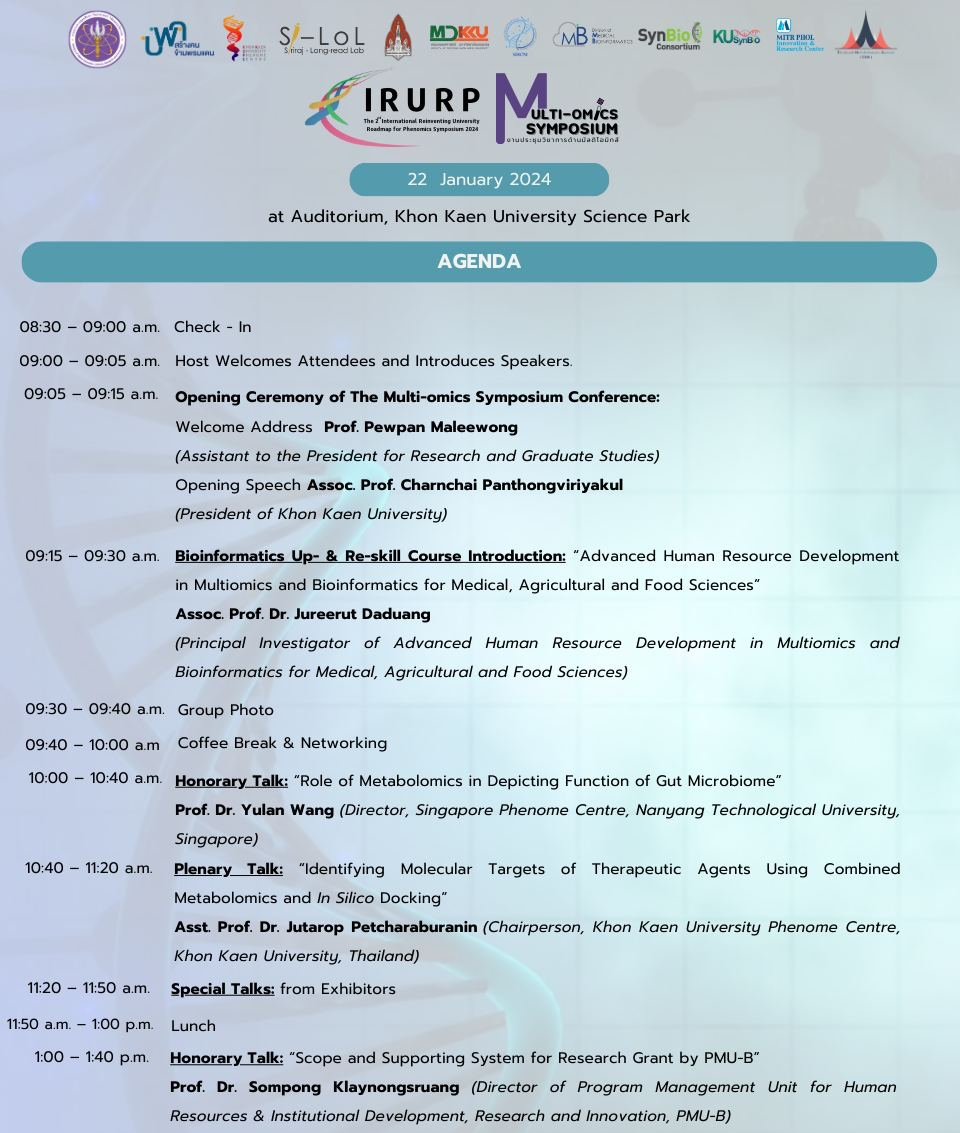
\includegraphics{Page/elements/img/Agenda/Agenda_1.jpg}\protect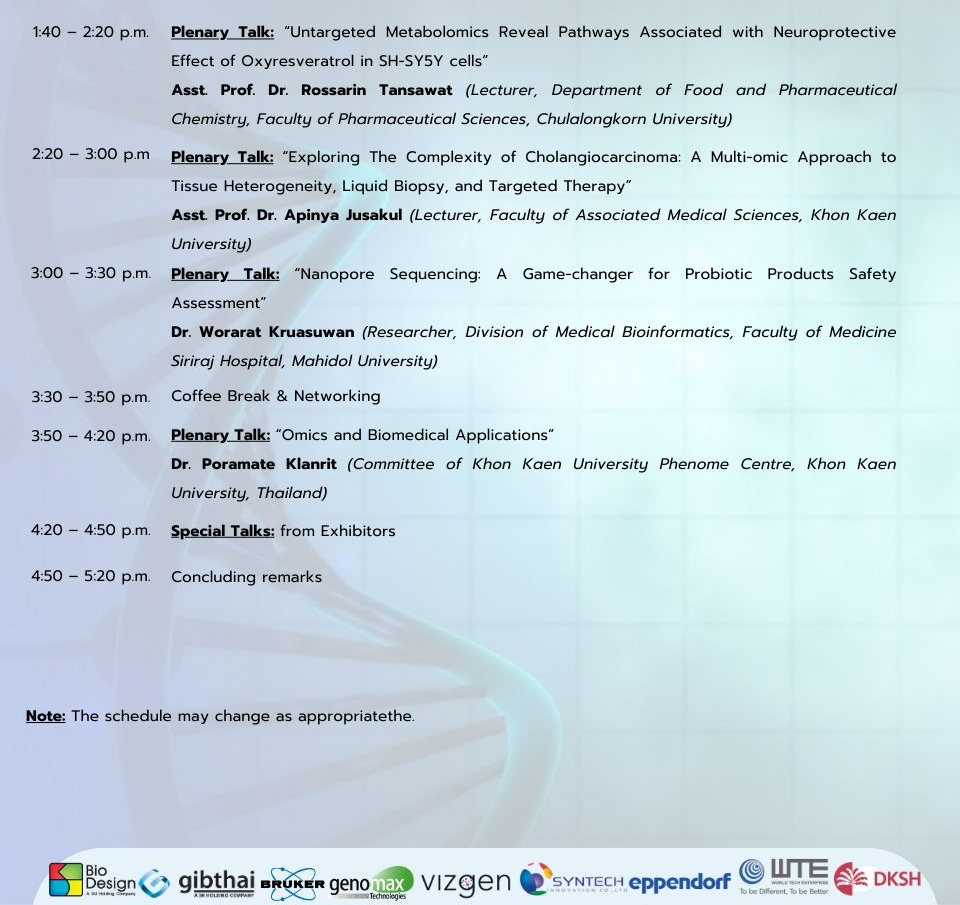
\includegraphics{Page/elements/img/Agenda/Agenda_2.jpg}}{}}\label{section-1}}

\hypertarget{time-table}{%
\subsection{\texorpdfstring{\href{Page/src/Time\%20table/Time_table.html}{Time
table}}{Time table}}\label{time-table}}

\begin{center}\rule{0.5\linewidth}{0.5pt}\end{center}

\hypertarget{exhibitors}{%
\subsection{\texorpdfstring{\textbf{Exhibitors}}{Exhibitors}}\label{exhibitors}}

\href{https://www.gibthai.com/}{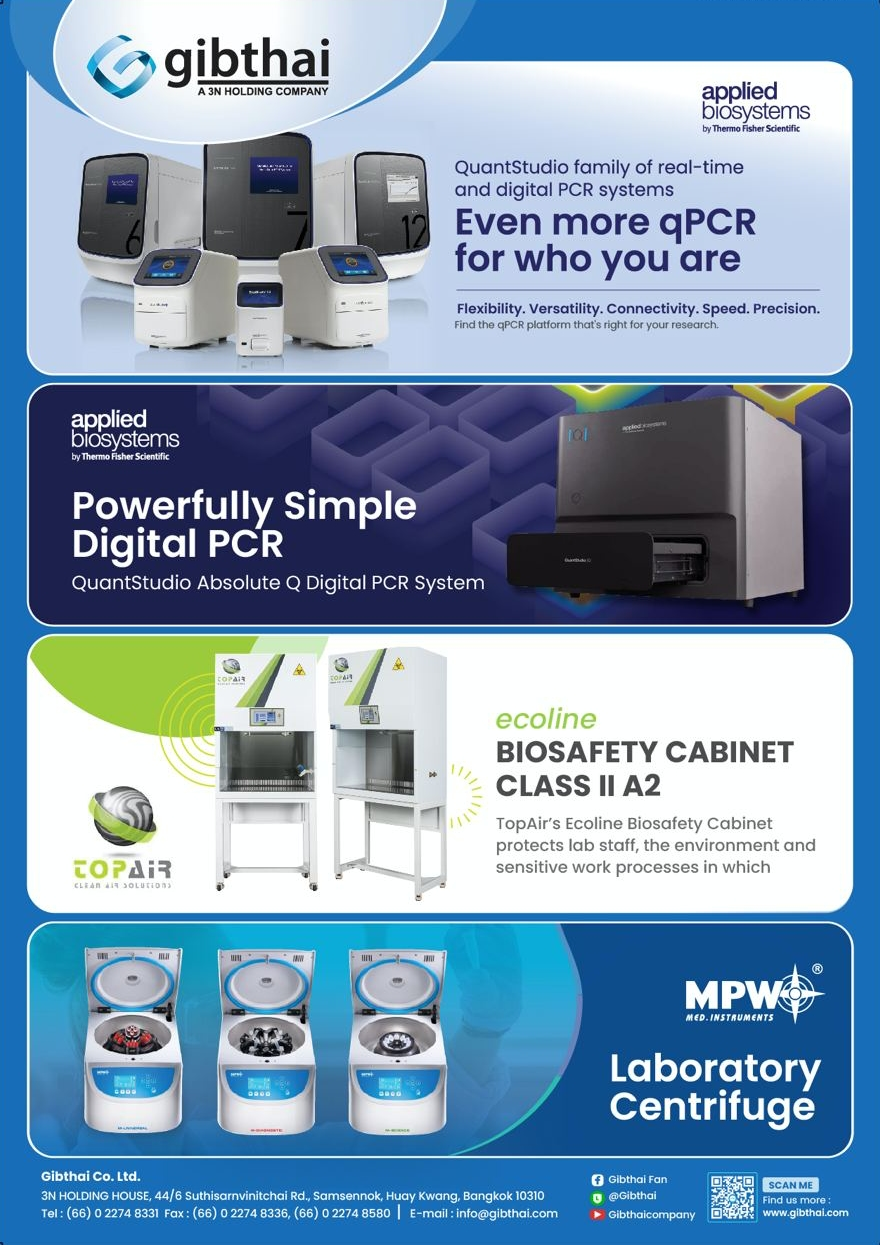
\includegraphics{./Page/elements/img/Exhibitors/Gibthai.jpg}}

\href{https://www.biodesign.co.th/}{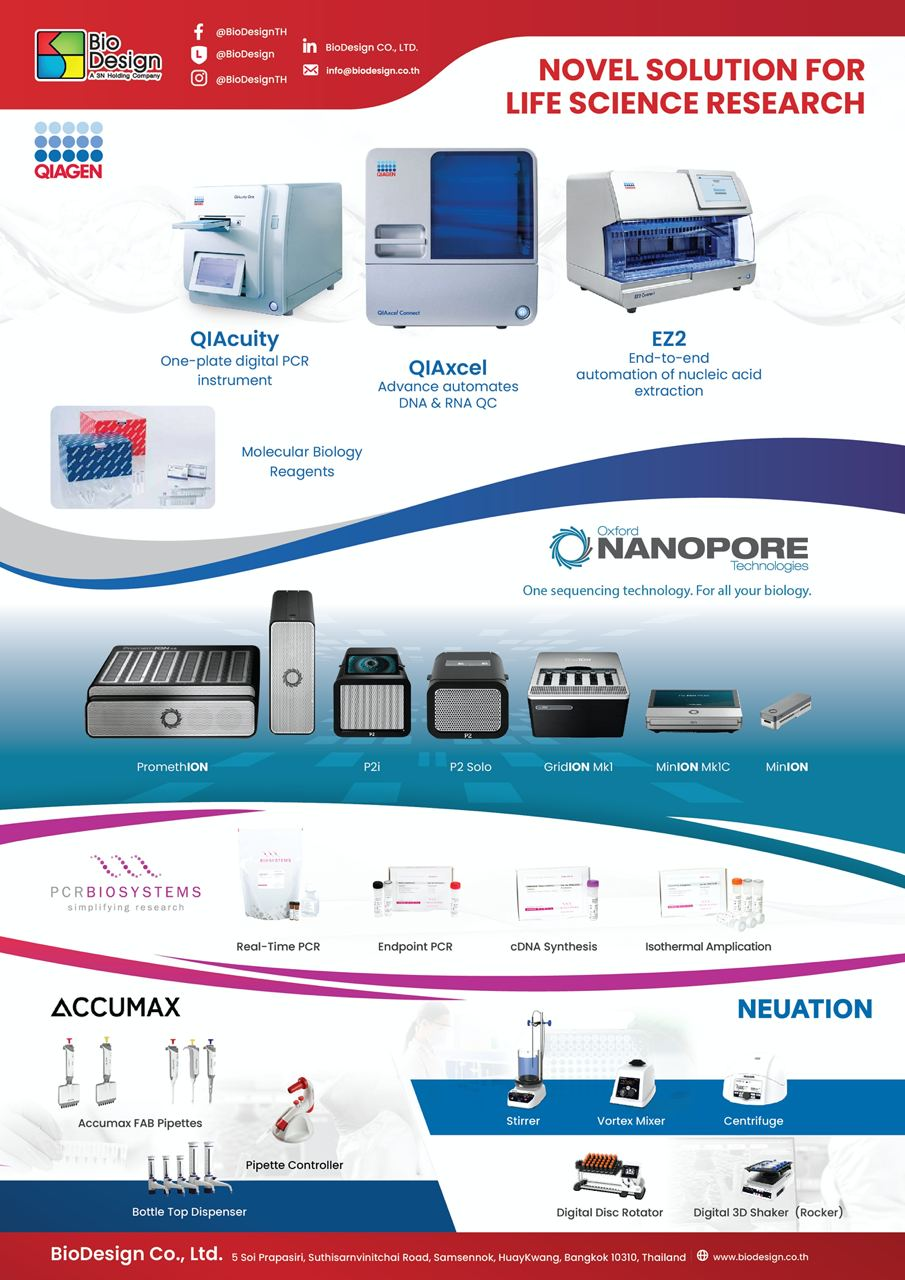
\includegraphics{./Page/elements/img/Exhibitors/Biodesign.jpeg}}

\href{https://www.bruker.com/en.html}{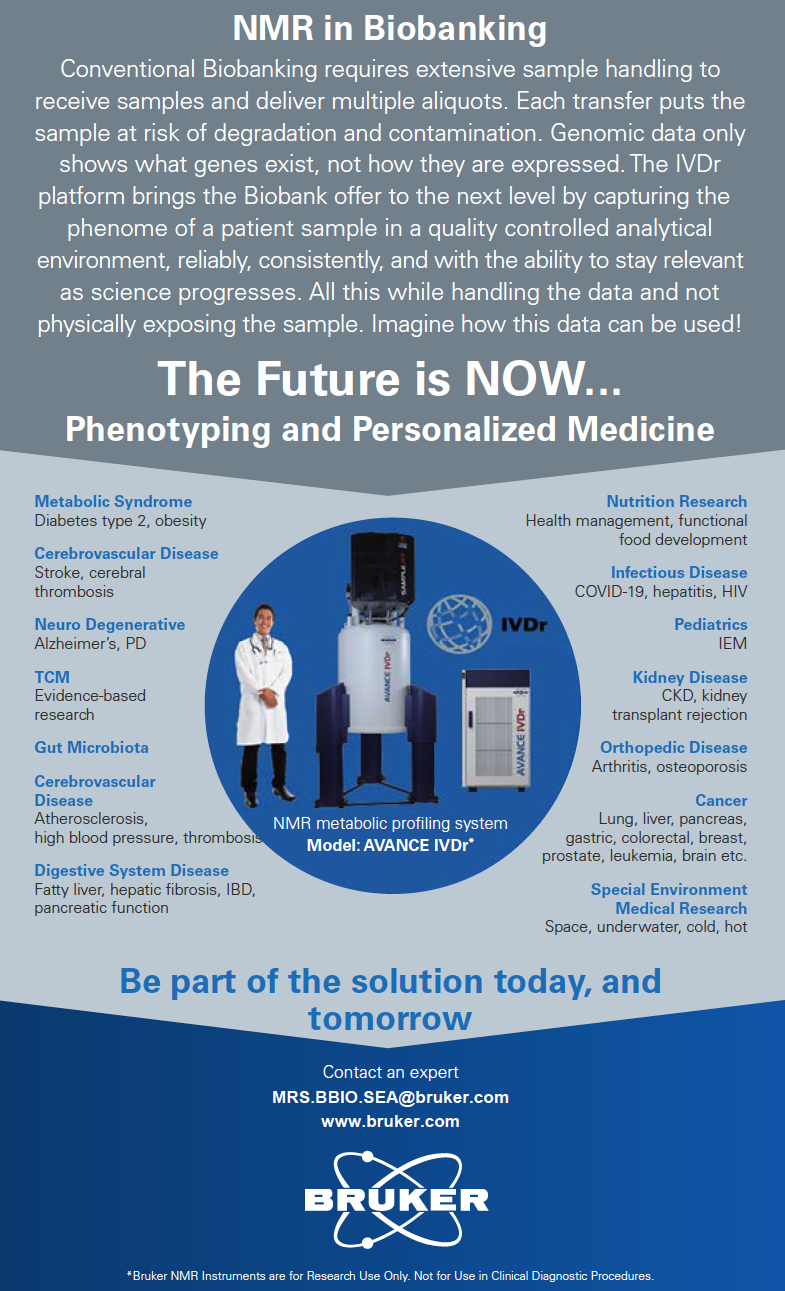
\includegraphics{./Page/elements/img/Exhibitors/Bruker.png}}

\href{https://www.genomaxtech.com}{
\includegraphics{./Page/elements/img/Exhibitors/Genomax.png}}

\href{https://worldtechenterprise.com}{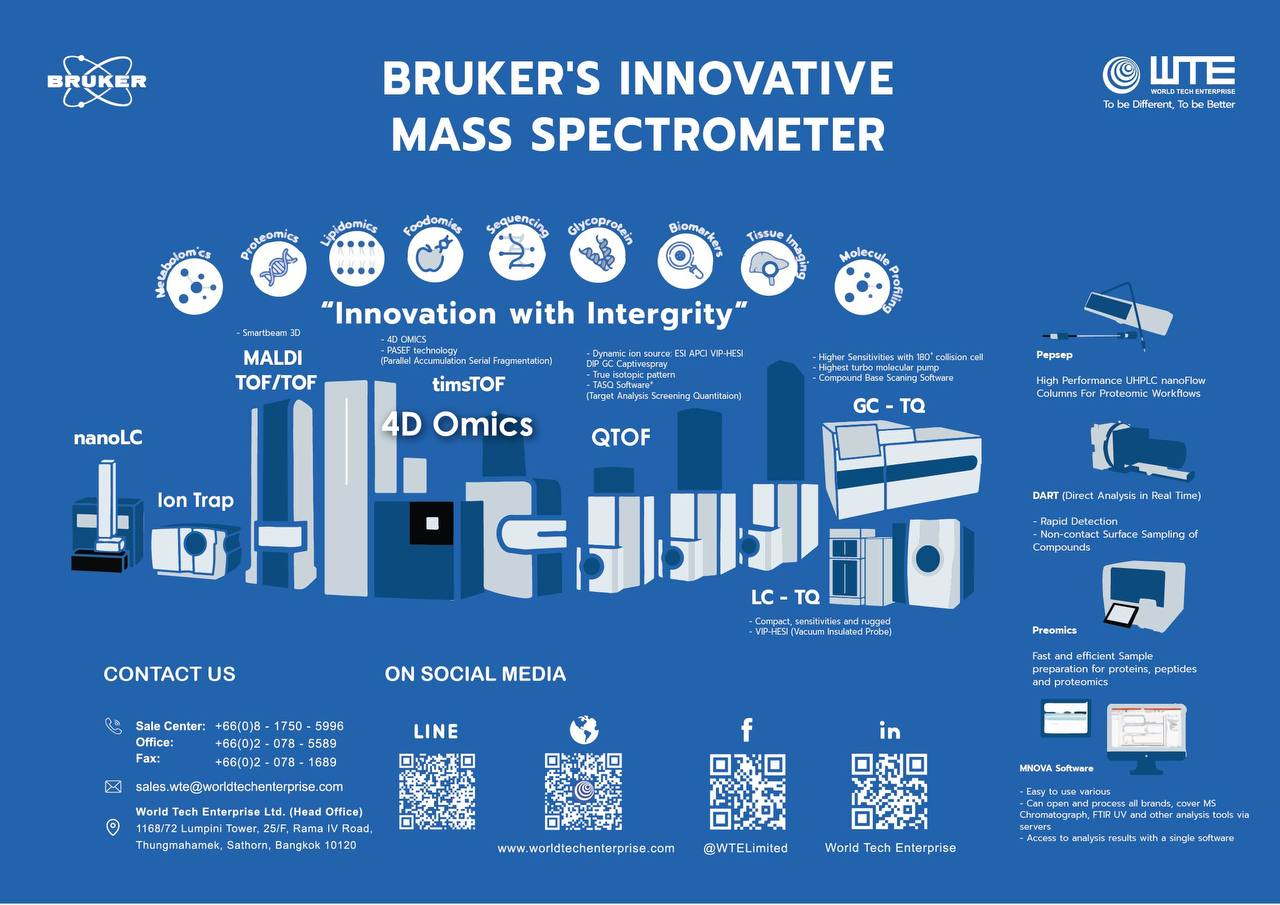
\includegraphics{./Page/elements/img/Exhibitors/WTE.jpeg}}

\href{https://www.dksh.com/th-en/home}{
\includegraphics{./Page/elements/img/Exhibitors/DKSH.png}}

\begin{center}\rule{0.5\linewidth}{0.5pt}\end{center}

\hypertarget{table-of-contents}{%
\subsection{Table of Contents}\label{table-of-contents}}

\begin{itemize}
\item
  \href{./Page/elements/contents/02\%20UNIX\%20session/Content/UNIX_Document.html}{UNIX}
\item
  \href{./Page/elements/contents/01\%20Experimental\%20design/Content/HandsOn.html}{Experimental
  design and analytical planing}
\item
  \href{./Page/elements/contents/03\%20R\%20session/Content/Rdocument.html}{R
  programing}
\item
  \href{./Page/elements/contents/04\%20Python/Content/Content.html}{Python}
\item
  \href{./Page/elements/contents/05\%20Genomics/Content/Content.html}{Genomics}
\item
  \href{./Page/elements/contents/06\%20Transcriptomics/Content/RNA.html}{Transcriptomics}
\item
  \href{./Page/elements/contents/07\%20Metabolomics/Content/Introduction.html}{Metabolomics}
\item
  \href{./Page/elements/contents/08\%20Proteomics/Content/Introduction.html}{Proteomics}
\item
  \href{./Page/elements/contents/09\%20CRISPR/Content/Content.html}{CRISPR}
\item
  \href{./Page/elements/contents/10\%20Microbiome/Content/Microbiome.html}{Microbiome}
\item
  \href{./Page/elements/contents/11\%20Data\%20integration/Content/Content.html}{Data
  integration}
\end{itemize}

\begin{center}\rule{0.5\linewidth}{0.5pt}\end{center}


\includegraphics{Page/elements/img/Logo/Logo_Multi-omics_2.png}
\includegraphics{Page/elements/img/Logo/Logo_Multi-omics_3.png}

\end{document}
